% questions.tex —— 2016 年·浙江卷·文科 · 题目内容片段（无答案）
% 由 tools/generate_projects.py 依来源总账自 2016/2016_数学真题_浙江文_试题.md 生成，勿手改（改源 MD 后重跑）


\gkpart{数学}

\begin{gktip}
\textbf{来源说明}：本题面依据固定源 PDF 两页 A3 页面逐题核对，原卷印刷页码 1029–1030。固定源不附答案、不印分值；本文件仅为题面规范源。源内中文标点一律为半角，本文件按项目约定统一为全角；源内异常一律照录并在 \texttt{.work} 版式文件中逐条登记（第 2 题三处平行记号「$\parallel$」在源文本层缺失、系矢量绘制，已照源补出——同卷「$\perp$」在文本层内，不得据此前推；第 4 题花括号为私用区分片；第 3 题四幅子图曲线照源矢量路径绘制、源内无文字标注；第 8 题图的角顶点在图外未绘出；第 14 题与第 19 题图为示意性画法，均照源复刻）。
\end{gktip}

\gkpart{一、选择题}

\begin{question}
\gkti{1}已知全集 \(U=\{1,2,3,4,5,6\}\)，集合 \(P=\{1,3,5\}\)，\(Q=\{1,2,4\}\)，则 \((\complement_U P)\cup Q=\)（　）

\begin{gkopts}(2)
\task （A）\(\{1\}\)
\task （B）\(\{3,5\}\)
\task （C）\(\{1,2,4,6\}\)
\task （D）\(\{1,2,3,4,5\}\)
\end{gkopts}

\end{question}
\begin{question}
\gkti{2}已知互相垂直的平面 \(\alpha\)，\(\beta\) 交于直线 \(l\)，若直线 \(m\)，\(n\) 满足 \(m\parallel\alpha\)，\(n\perp\beta\)，则（　）

\begin{gkopts}(2)
\task （A）\(m\parallel l\)
\task （B）\(m\parallel n\)
\task （C）\(n\perp l\)
\task （D）\(m\perp n\)
\end{gkopts}

\Needspace{0.4\textheight}
\end{question}
\begin{question}
\gkti{3}函数 \(y=\sin x^{2}\) 的图象是（　）
\nopagebreak[4]
\begin{center}% 第 3 题四图像：按固定源 PDF 矢量路径换算（1 pt → 0.03515 cm）。
% 原点取 (A) 面板原点（源页 (150.89, 350.45) pt），y 向上；1 单位 = 25.5 pt（横纵同比例）。
% 四面板原点（相对本坐标系）：(A)(0,0)、(B)(169.57,0)、(C)(−0.30,−93.30)、(D)(170.16,−93.30)。
% 每面板：y 轴自原点下 38.25 上至箭头尖点 38.25；x 轴左 63.76 右至箭头尖点 63.76；
% y 轴刻度线 (0,25.5)–(3.06,25.5) 标「1」；x 轴刻度线在 ±40.06（=π/2×25.5）各长 3.06。
% 曲线线宽 0.8pt（源为轴 0.398 的 2 倍）；四曲线形状经矢量采样数值拟合为
% (A) sign(x)·sin²x、(B) |sin x|、(C) sign(x)·sin(x²)、(D) sin(x²)
% （源内四图无函数式标注，拟合残差 ≤0.003 单位；照此绘制，不写入题面）。
% 轴标签 y/x/O、刻度「1」与分式「−π/2」「π/2」按源字形框中心显式定位；
% (C) 面板左标签整组位于 x 轴上方（源内如此，照录）；选项标号 (A)(B)(C)(D) 在各面板下方源位。
% 【修复轮修正】初版按字框中心定位使「−π/2」「π/2」的 π 与 x 轴线墨迹相融（试题版 P1
% figure_label 600 dpi 连通域查出：π 腿跨轴、与轴同属一分量）。按源墨迹实测重定位：
% 源内轴下标签的 π 顶横距轴心 3.7 pt（600 dpi 行测 31 px/8.333），2 底距轴 ≥2.2 pt——
% 七个轴下标签整体下移 4.86 pt、C 面板轴上标签上移 2.0 pt（其余水平位置不变）。
\begin{tikzpicture}[line cap=round,line join=round,font=\small,x=0.03515cm,y=0.03515cm]
% ===== 面板 (A) =====
\draw[->] (0,-38.25)--(0,38.25);
\draw[->] (-63.76,0)--(63.76,0);
\draw (0,25.5)--(3.06,25.5);
\draw (-40.06,0)--(-40.06,3.06);
\draw (40.06,0)--(40.06,3.06);
\draw[line width=0.8pt] plot[domain=-2:2,samples=201] ({25.5*\x},{25.5*sign(\x)*sin(deg(\x))*sin(deg(\x))});
\node[anchor=center,inner sep=0] at (-6.59,39.62) {\(y\)};
\node[anchor=center,inner sep=0] at (6.38,24.72) {\(1\)};
\node[anchor=center,inner sep=0] at (-7.94,-8.28) {\(O\)};
\node[anchor=center,inner sep=0] at (63.83,-5.63) {\(x\)};
\node[anchor=center,inner sep=0] at (-40.64,-13.23) {\(-\dfrac{\pi}{2}\)};
\node[anchor=center,inner sep=0] at (40.00,-13.73) {\(\dfrac{\pi}{2}\)};
% ===== 面板 (B)（右移 169.57）=====
\begin{scope}[shift={(169.57,0)}]
\draw[->] (0,-38.25)--(0,38.25);
\draw[->] (-63.76,0)--(63.76,0);
\draw (0,25.5)--(3.06,25.5);
\draw (-40.06,0)--(-40.06,3.06);
\draw (40.06,0)--(40.06,3.06);
\draw[line width=0.8pt] plot[domain=-2:2,samples=201] ({25.5*\x},{25.5*abs(sin(deg(\x)))});
\node[anchor=center,inner sep=0] at (-6.53,39.62) {\(y\)};
\node[anchor=center,inner sep=0] at (6.45,24.72) {\(1\)};
\node[anchor=center,inner sep=0] at (-7.88,-8.28) {\(O\)};
\node[anchor=center,inner sep=0] at (63.90,-5.63) {\(x\)};
\node[anchor=center,inner sep=0] at (-40.67,-13.23) {\(-\dfrac{\pi}{2}\)};
\node[anchor=center,inner sep=0] at (40.07,-13.73) {\(\dfrac{\pi}{2}\)};
\end{scope}
% ===== 面板 (C)（下移 93.30，左移 0.30）=====
\begin{scope}[shift={(-0.30,-93.30)}]
\draw[->] (0,-38.25)--(0,38.25);
\draw[->] (-63.76,0)--(63.76,0);
\draw (0,25.5)--(3.06,25.5);
\draw (-40.06,0)--(-40.06,3.06);
\draw (40.06,0)--(40.06,3.06);
\draw[line width=0.8pt] plot[domain=-2:2,samples=201] ({25.5*\x},{25.5*sign(\x)*sin(deg(\x*\x))});
\node[anchor=center,inner sep=0] at (-6.59,39.59) {\(y\)};
\node[anchor=center,inner sep=0] at (6.39,24.69) {\(1\)};
\node[anchor=center,inner sep=0] at (-7.94,-8.31) {\(O\)};
\node[anchor=center,inner sep=0] at (63.84,-5.66) {\(x\)};
\node[anchor=center,inner sep=0] at (-40.63,11.75) {\(-\dfrac{\pi}{2}\)};
\node[anchor=center,inner sep=0] at (40.01,-13.76) {\(\dfrac{\pi}{2}\)};
\end{scope}
% ===== 面板 (D)（下移 93.30，右移 170.16）=====
\begin{scope}[shift={(170.16,-93.30)}]
\draw[->] (0,-38.25)--(0,38.25);
\draw[->] (-63.76,0)--(63.76,0);
\draw (0,25.5)--(3.06,25.5);
\draw (-40.06,0)--(-40.06,3.06);
\draw (40.06,0)--(40.06,3.06);
\draw[line width=0.8pt] plot[domain=-2:2,samples=201] ({25.5*\x},{25.5*sin(deg(\x*\x))});
\node[anchor=center,inner sep=0] at (-6.53,39.59) {\(y\)};
\node[anchor=center,inner sep=0] at (6.45,24.69) {\(1\)};
\node[anchor=center,inner sep=0] at (-7.88,-8.31) {\(O\)};
\node[anchor=center,inner sep=0] at (63.90,-5.66) {\(x\)};
\node[anchor=center,inner sep=0] at (-40.60,-13.26) {\(-\dfrac{\pi}{2}\)};
\node[anchor=center,inner sep=0] at (40.07,-13.76) {\(\dfrac{\pi}{2}\)};
\end{scope}
% ===== 选项标号（照源字形框中心；置于各面板下方）=====
\node[anchor=center,inner sep=0] at (-75.44,-35.28) {(A)};
\node[anchor=center,inner sep=0] at (94.42,-35.28) {(B)};
\node[anchor=center,inner sep=0] at (-75.58,-128.62) {(C)};
\node[anchor=center,inner sep=0] at (94.71,-128.62) {(D)};
\end{tikzpicture}
\end{center}
\nopagebreak[4]
\end{question}
\begin{question}
\gkti{4}若平面区域
\nopagebreak[4]
\[
\begin{cases}
x+y-3\geqslant 0,\\
2x-y-3\leqslant 0,\\
x-2y+3\geqslant 0
\end{cases}
\]
夹在两条斜率为 1 的平行直线之间，则这两条平行直线间的距离的最小值是（　）

\begin{gkopts}(1)
\task （A）\(\dfrac{3\sqrt{5}}{5}\)
\task （B）\(\sqrt{2}\)
\task （C）\(\dfrac{3\sqrt{2}}{2}\)
\task （D）\(\sqrt{5}\)
\end{gkopts}

\end{question}
\begin{question}
\gkti{5}已知 \(a\)，\(b>0\)，且 \(a\neq1\)，\(b\neq1\)，若 \(\log_a b>1\)，则（　）

\begin{gkopts}(2)
\task （A）\((a-1)(b-1)<0\)
\task （B）\((a-1)(a-b)>0\)
\task （C）\((b-1)(b-a)<0\)
\task （D）\((b-1)(b-a)>0\)
\end{gkopts}

\end{question}
\begin{question}
\gkti{6}已知函数 \(f(x)=x^{2}+bx\)，则“\(b<0\)”是“\(f(f(x))\) 的最小值与 \(f(x)\) 的最小值相等”的（　）

\begin{gkopts}(2)
\task （A）充分不必要条件
\task （B）必要不充分条件
\task （C）充分必要条件
\task （D）既不充分也不必要条件
\end{gkopts}

\end{question}
\begin{question}
\gkti{7}已知函数 \(f(x)\) 满足：\(f(x)\geqslant|x|\) 且 \(f(x)\geqslant2^{x}\)，\(x\in\mathbf{R}\)。（　）

（A）若 \(f(a)\leqslant|b|\)，则 \(a\leqslant b\)　（B）若 \(f(a)\leqslant2^{b}\)，则 \(a\leqslant b\)

（C）若 \(f(a)\geqslant|b|\)，则 \(a\geqslant b\)　（D）若 \(f(a)\geqslant2^{b}\)，则 \(a\geqslant b\)

\Needspace{0.4\textheight}
\end{question}
\begin{question}
\gkti{8}如图，点列 \(\{A_{n}\}\)，\(\{B_{n}\}\) 分别在某锐角的两边上，且 \(|A_{n}A_{n+1}|=|A_{n+1}A_{n+2}|\)，\(A_{n}\neq A_{n+2}\)，\(n\in\mathbf{N}^{*}\)，\(|B_{n}B_{n+1}|=|B_{n+1}B_{n+2}|\)，\(B_{n}\neq B_{n+2}\)，\(n\in\mathbf{N}^{*}\)（\(P\neq Q\) 表示点 \(P\) 与 \(Q\) 不重合）。若 \(d_{n}=|A_{n}B_{n}|\)，\(S_{n}\) 为 \(\triangle A_{n}B_{n}B_{n+1}\) 的面积，则（　）
\nopagebreak[4]
\begin{center}% 第 8 题点列图：按固定源 PDF 矢量路径换算（1 pt → 0.03515 cm）。
% 原点取下边水平线的左端（源页 (533.34, 203.23) pt），y 向上。
% 两条边（角的两边）：水平线 y=0 与斜线（自 (0.37,20.99) 至 (103.90,78.47)）；
% 角的顶点在图外有意未绘出（两线左端被同一竖直截断线切齐，端头纵向相距 20.99 pt）。
% 三个 10% 灰填充三角形 S1/S2/Sn（顶点按源路径逐点换算）；
% 点列 A1..A(n+1) 在斜线上、B1..B(n+1) 在水平线上；4 组省略号（A 线 1、S 行 2、B 行 1）。
% 全部标签按源字形框中心显式坐标定位。
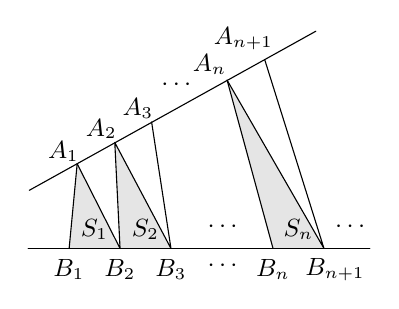
\begin{tikzpicture}[line cap=round,line join=round,font=\small,x=0.03515cm,y=0.03515cm]
% ===== 两条边 =====
\draw (0,0)--(123.43,0);               % 水平线（下边，B 点列所在）
\draw (0.37,20.99)--(103.90,78.47);    % 斜线（上边，A 点列所在）
% ===== 填充三角形（fill-opacity 0.1）=====
\fill[black,fill opacity=0.1] (17.68,30.58)--(14.78,-0.01)--(33.17,-0.01)--cycle;
\fill[black,fill opacity=0.1] (31.27,38.28)--(33.17,-0.01)--(51.56,-0.01)--cycle;
\fill[black,fill opacity=0.1] (71.84,60.79)--(88.43,0.01)--(106.83,0.01)--cycle;
% ===== 线段 =====
\draw (17.68,30.58)--(14.78,-0.01);                       % A1B1
\draw (17.68,30.58)--(33.17,-0.01)--(31.27,38.28)--(51.56,-0.01)--(44.57,45.68);  % A1→B2→A2→B3→A3
\draw (71.84,60.79)--(88.43,0.01);                        % AnBn
\draw (71.84,60.79)--(106.83,0.01)--(85.43,68.19);        % An→Bn+1→An+1
% ===== 标签（照源字形框中心，显式坐标）=====
\node[anchor=center,inner sep=0] at (12.71,34.93) {\(A_{1}\)};
\node[anchor=center,inner sep=0] at (26.35,43.11) {\(A_{2}\)};
\node[anchor=center,inner sep=0] at (39.62,50.48) {\(A_{3}\)};
\node[anchor=center,inner sep=0] at (53.51,59.21) {\(\cdots\)};
\node[anchor=center,inner sep=0] at (65.48,66.56) {\(A_{n}\)};
\node[anchor=center,inner sep=0] at (77.72,75.76) {\(A_{n+1}\)};
\node[anchor=center,inner sep=0] at (14.70,-7.57) {\(B_{1}\)};
\node[anchor=center,inner sep=0] at (33.12,-7.57) {\(B_{2}\)};
\node[anchor=center,inner sep=0] at (51.55,-7.57) {\(B_{3}\)};
\node[anchor=center,inner sep=0] at (70.23,-6.14) {\(\cdots\)};
\node[anchor=center,inner sep=0] at (88.41,-7.57) {\(B_{n}\)};
\node[anchor=center,inner sep=0] at (110.82,-7.57) {\(B_{n+1}\)};
\node[anchor=center,inner sep=0] at (23.91,6.82) {\(S_{1}\)};
\node[anchor=center,inner sep=0] at (42.34,6.82) {\(S_{2}\)};
\node[anchor=center,inner sep=0] at (70.23,7.81) {\(\cdots\)};
\node[anchor=center,inner sep=0] at (97.63,6.82) {\(S_{n}\)};
\node[anchor=center,inner sep=0] at (116.30,7.81) {\(\cdots\)};
\end{tikzpicture}
\end{center}
\nopagebreak[4]
\begin{gkopts}(2)
\task （A）\(\{S_{n}\}\) 是等差数列
\task （B）\(\{S_{n}^{2}\}\) 是等差数列
\task （C）\(\{d_{n}\}\) 是等差数列
\task （D）\(\{d_{n}^{2}\}\) 是等差数列
\end{gkopts}

\end{question}
\gkpart{二、填空题}

\Needspace{0.4\textheight}
\begin{question}
\gkti{9}某几何体的三视图如图所示（单位：cm），则该几何体的表面积是\gkblank{}cm²，体积是\gkblank{}cm³。
\nopagebreak[4]
\begin{center}% 第 9 题三视图：按固定源 PDF 矢量路径换算（1 pt → 0.03515 cm）。
% 原点取正视图左下角（源页 (531.30, 382.71) pt），y 向上。网格 25.5 pt = 2 cm。
% 正视图：L 形（左柱 2×2 在下、右柱 2×4 通高；中竖贯通、中横仅左半——按源矢量路径复核）；
% 侧视图：与正视图互为镜像（左柱通高、右柱仅下段），右柱右棱下半为虚线（源内线型如此，照录）；
% 俯视图：左列满深 2×4、右上 2×2 正方形。
% 尺寸标注：横向 4 条（正视图两格 + 侧视图两格）@y=56.10、竖向 2 条 @x=56.10（均两段让位给数字）；
% 6 条竖直刻度线、3 条水平刻度线；12 个实心箭头（一律朝外）；「2」「正视图」「侧视图」「俯视图」共 9 个标签（照源字形框中心）。
\begin{tikzpicture}[line cap=round,line join=round,font=\small,x=0.03515cm,y=0.03515cm]
% ===== 正视图（左格）=====
\draw (0,0)--(51,0)--(51,51)--(25.5,51)--(25.5,25.5)--(0,25.5)--cycle;
\draw (25.5,0)--(25.5,25.5);                 % 中竖下半（实线）
% ===== 侧视图（右格，右移 76.5）=====
\draw (76.5,0)--(127.51,0)--(127.51,25.5)--(102,25.5)--(102,51)--(76.5,51)--cycle;
\draw (76.5,25.5)--(102,25.5);               % 中横左半（实线）
\draw[dash pattern=on 2.99pt off 2.99pt] (102,0)--(102,25.5);  % 中竖下半（虚线，照源）
% ===== 俯视图 =====
\draw (0,-25.5)--(25.5,-25.5)--(25.5,-76.51)--(0,-76.51)--cycle;   % 左列满深
\draw (25.5,-25.5)--(51,-25.5)--(51,-51.01)--(25.5,-51.01);        % 右上正方形（第四边与左列右边重合）
% ===== 尺寸线（横向 4 条 @y=56.10，两段让位）=====
\draw (3.58,56.10)--(21.91,56.10);   \draw (29.08,56.10)--(47.41,56.10);       % 正视图两格
\draw (80.09,56.10)--(98.42,56.10);  \draw (105.59,56.10)--(123.92,56.10);     % 侧视图两格
% ===== 尺寸线（竖向 2 条 @x=56.10，两段让位）=====
\draw (56.10,29.09)--(56.10,47.42);  % 上段（高 2）
\draw (56.10,3.58)--(56.10,21.91);   % 下段（高 2）
% ===== 竖直刻度线（6 条，@y 53.55–61.20）=====
\draw (0,53.55)--(0,61.20);         \draw (25.5,53.55)--(25.5,61.20);
\draw (51,53.55)--(51,61.20);       \draw (76.5,53.55)--(76.5,61.20);
\draw (102,53.55)--(102,61.20);     \draw (127.51,53.55)--(127.51,61.20);
% ===== 水平刻度线（3 条，@x 53.55–61.20）=====
\draw (53.55,0)--(61.20,0);
\draw (53.55,25.5)--(61.20,25.5);
\draw (53.55,51)--(61.20,51);
% ===== 实心箭头（12 个，底 2.98 长 3.98，一律朝外）=====
\fill (0,56.10)--(3.98,54.61)--(3.98,57.59)--cycle;             % 正左格：左端←
\fill (25.5,56.10)--(21.52,54.61)--(21.52,57.59)--cycle;       % 正左格：右端→
\fill (25.5,56.10)--(29.48,54.61)--(29.48,57.59)--cycle;       % 正右格：左端←
\fill (51,56.10)--(47.02,54.61)--(47.02,57.59)--cycle;         % 正右格：右端→
\fill (76.5,56.10)--(80.48,54.61)--(80.48,57.59)--cycle;       % 侧左格：左端←
\fill (102,56.10)--(98.02,54.61)--(98.02,57.59)--cycle;        % 侧左格：右端→
\fill (102,56.10)--(105.98,54.61)--(105.98,57.59)--cycle;      % 侧右格：左端←
\fill (127.51,56.10)--(123.53,54.61)--(123.53,57.59)--cycle;   % 侧右格：右端→
\fill (56.10,51)--(54.61,47.02)--(57.59,47.02)--cycle;         % 上段：上端↑
\fill (56.10,25.5)--(54.61,29.48)--(57.59,29.48)--cycle;       % 上段：下端↓
\fill (56.10,25.5)--(54.61,21.52)--(57.59,21.52)--cycle;       % 下段：上端↑
\fill (56.10,0)--(54.61,3.98)--(57.59,3.98)--cycle;            % 下段：下端↓
% ===== 标签（照源字形框中心，显式坐标）=====
\node[anchor=center,inner sep=0] at (12.96,60.43) {\(2\)};
\node[anchor=center,inner sep=0] at (38.47,60.43) {\(2\)};
\node[anchor=center,inner sep=0] at (89.49,60.43) {\(2\)};
\node[anchor=center,inner sep=0] at (115.01,60.43) {\(2\)};
\node[anchor=center,inner sep=0] at (61.43,37.46) {\(2\)};
\node[anchor=center,inner sep=0] at (61.43,11.95) {\(2\)};
\node[anchor=center,inner sep=0] at (25.71,-12.21) {正视图};
\node[anchor=center,inner sep=0] at (102.24,-12.19) {侧视图};
\node[anchor=center,inner sep=0] at (25.71,-88.67) {俯视图};
\end{tikzpicture}
\end{center}
\nopagebreak[4]
\end{question}
\begin{question}
\gkti{10}已知 \(a\in\mathbf{R}\)，方程 \(a^{2}x^{2}+(a+2)y^{2}+4x+8y+5a=0\) 表示圆，则圆心坐标是\gkblank{}，半径是\gkblank{}。

\end{question}
\begin{question}
\gkti{11}已知 \(2\cos^{2}x+\sin 2x=A\sin(\omega x+\varphi)+B\)（\(A>0\)），则 \(A=\)\gkblank{}，\(B=\)\gkblank{}。

\end{question}
\begin{question}
\gkti{12}设函数 \(f(x)=x^{3}+3x^{2}+1\)，已知 \(a\neq0\)，且 \(f(x)-f(a)=(x-b)(x-a)^{2}\)，\(x\in\mathbf{R}\)，则实数 \(a=\)\gkblank{}，\(b=\)\gkblank{}。

\end{question}
\begin{question}
\gkti{13}设双曲线 \(x^{2}-\dfrac{y^{2}}{3}=1\) 的左，右焦点分别为 \(F_{1}\)，\(F_{2}\)，若点 \(P\) 在双曲线上，且 \(\triangle F_{1}PF_{2}\) 为锐角三角形，则 \(|PF_{1}|+|PF_{2}|\) 的取值范围是\gkblank{}。

\Needspace{0.4\textheight}
\end{question}
\begin{question}
\gkti{14}如图，已知平面四边形 \(ABCD\)，\(AB=BC=3\)，\(CD=1\)，\(AD=\sqrt{5}\)，\(\angle ADC=90^{\circ}\)。沿直线 \(AC\) 将 \(\triangle ACD\) 翻折成 \(\triangle ACD'\)，直线 \(AC\) 与 \(BD'\) 所成角的余弦的最大值是\gkblank{}。
\nopagebreak[4]
\begin{center}% 第 14 题翻折图：按固定源 PDF 矢量路径换算（1 pt → 0.03515 cm）。
% 原点取 C 点（源页 (565.39, 736.24) pt），y 向上。
% 平面四边形 ABCD：AC 为翻折轴（实线）；D 到 A、C 两边为虚线（翻折前位置）；
% 翻折后 D′ 到 A、C 两边为实线；BA、BC 实线。虚实归属由各路径 stroke-dasharray 直接判定。
% 各顶点旁标注 A/B/C/D/D′（照源字形框中心）。源图为示意（不按比例），照源复刻。
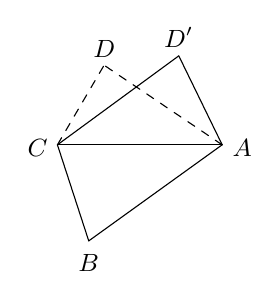
\begin{tikzpicture}[line cap=round,line join=round,font=\small,x=0.03515cm,y=0.03515cm]
\draw (59.51,0)--(0,0);                % A–C（翻折轴）
\draw (11.31,-34.71)--(0,0);           % B–C
\draw (11.31,-34.71)--(59.51,0);       % B–A
\draw (0,0)--(43.84,32.14);            % C–D′
\draw (59.51,0)--(43.84,32.14);        % A–D′
\draw[dash pattern=on 2.99pt off 2.99pt] (0,0)--(16.86,28.76);      % C–D（虚线，翻折前位置）
\draw[dash pattern=on 2.99pt off 2.99pt] (59.51,0)--(16.86,28.76);  % A–D（虚线，翻折前位置）
% ===== 标签（照源字形框中心，显式坐标）=====
\node[anchor=center,inner sep=0] at (66.72,-1.14) {\(A\)};
\node[anchor=center,inner sep=0] at (11.27,-42.84) {\(B\)};
\node[anchor=center,inner sep=0] at (-7.13,-1.14) {\(C\)};
\node[anchor=center,inner sep=0] at (16.94,34.61) {\(D\)};
\node[anchor=center,inner sep=0] at (43.82,38.74) {\(D'\)};
\end{tikzpicture}
\end{center}
\nopagebreak[4]
\end{question}
\begin{question}
\gkti{15}已知平面向量 \(\boldsymbol{a}\)，\(\boldsymbol{b}\)，\(|\boldsymbol{a}|=1\)，\(|\boldsymbol{b}|=2\)，\(\boldsymbol{a}\cdot\boldsymbol{b}=1\)。若 \(\boldsymbol{e}\) 为平面单位向量，则 \(|\boldsymbol{a}\cdot\boldsymbol{e}|+|\boldsymbol{b}\cdot\boldsymbol{e}|\) 的最大值是\gkblank{}。

\end{question}
\gkpart{三、解答题}

\begin{question}
\gkti{16}在 \(\triangle ABC\) 中，内角 \(A\)，\(B\)，\(C\) 所对的边分别为 \(a\)，\(b\)，\(c\)。已知 \(b+c=2a\cos B\)。

（1） 证明：\(A=2B\)；

（2） 若 \(\cos B=\dfrac{2}{3}\)，求 \(\cos C\) 的值。

\end{question}
\begin{question}
\gkti{17}设数列 \(\{a_{n}\}\) 的前 \(n\) 项和为 \(S_{n}\)。已知 \(S_{2}=4\)，\(a_{n+1}=2S_{n}+1\)，\(n\in\mathbf{N}^{*}\)。

（1） 求通项公式 \(a_{n}\)；

（2） 求数列 \(\{|a_{n}-n-2|\}\) 的前 \(n\) 项和。

\Needspace{0.4\textheight}
\end{question}
\begin{question}
\gkti{18}如图，在三棱台 \(ABC-DEF\) 中，平面 \(BCFE\perp\) 平面 \(ABC\)，\(\angle ACB=90^{\circ}\)，\(BE=EF=FC=1\)，\(BC=2\)，\(AC=3\)。

（1） 求证：\(BF\perp\) 平面 \(ACFD\)；

（2） 求直线 \(BD\) 与平面 \(ACFD\) 所成角的余弦值。
\nopagebreak[4]
\begin{center}% 第 18 题三棱台：按固定源 PDF 矢量路径换算（1 pt → 0.03515 cm）。
% 原点取 A 点（源页 (237.39, 177.27) pt），y 向上。
% 上底面 D-E-F（D 左上、F 右上、E 居中略低）、下底面 A-B-C（A 左、C 右、B 下方）。
% 实线 10 条：侧棱 AD/EB/FC、上底 DF/DE/EF、下底 BA/BC、辅助线 DB（第 (2) 问所问直线）与侧面 BCFE 对角线 FB；
% 虚线 1 条：AC（被遮挡的下底棱，stroke-dasharray 直接判定）。各顶点旁标注 A/B/C/D/E/F（照源字形框中心）。
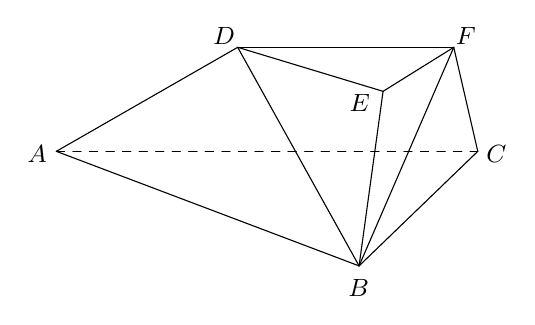
\begin{tikzpicture}[line cap=round,line join=round,font=\small,x=0.03515cm,y=0.03515cm]
\draw (0,0)--(65.52,37.58);             % A–D（侧棱）
\draw (65.52,37.58)--(143.57,37.58);    % D–F（上底棱，水平）
\draw (65.52,37.58)--(118.04,21.68);    % D–E（上底棱）
\draw (118.04,21.68)--(143.57,37.58);   % E–F（上底棱）
\draw (143.57,37.58)--(152.25,0);       % F–C（侧棱）
\draw (118.04,21.68)--(109.37,-41.38);  % E–B（侧棱）
\draw (65.52,37.58)--(109.37,-41.38);   % D–B（辅助线）
\draw (143.57,37.58)--(109.37,-41.38);  % F–B（侧面 BCFE 对角线）
\draw (0,0)--(109.37,-41.38);           % A–B（下底棱）
\draw (109.37,-41.38)--(152.25,0);      % B–C（下底棱）
\draw[dash pattern=on 2.99pt off 2.99pt] (0,0)--(152.25,0);  % A–C（虚线，被遮挡）
% ===== 标签（照源字形框中心，显式坐标）=====
\node[anchor=center,inner sep=0] at (-6.88,-0.92) {\(A\)};
\node[anchor=center,inner sep=0] at (109.24,-49.35) {\(B\)};
\node[anchor=center,inner sep=0] at (158.99,-0.92) {\(C\)};
\node[anchor=center,inner sep=0] at (60.56,41.60) {\(D\)};
\node[anchor=center,inner sep=0] at (109.59,17.33) {\(E\)};
\node[anchor=center,inner sep=0] at (147.92,41.60) {\(F\)};
\end{tikzpicture}
\end{center}
\nopagebreak[4]
\Needspace{0.4\textheight}
\end{question}
\begin{question}
\gkti{19}如图，设抛物线 \(y^{2}=2px\)（\(p>0\)）的焦点为 \(F\)，抛物线上的点 \(A\) 到 \(y\) 轴的距离等于 \(|AF|-1\)。

（1） 求 \(p\) 的值；

（2） 若直线 \(AF\) 交抛物线于另一点 \(B\)，过 \(B\) 与 \(x\) 轴平行的直线和过 \(F\) 与 \(AB\) 垂直的直线交于点 \(N\)，\(AN\) 与 \(x\) 轴交于点 \(M\)。求 \(M\) 的横坐标的取值范围。
\nopagebreak[4]
\begin{center}% 第 19 题抛物线图：按固定源 PDF 矢量路径换算（1 pt → 0.03515 cm）。
% 原点取 O（抛物线顶点，源页 (670.24, 226.48) pt），y 向上。
% 抛物线线宽 0.8pt（其余图元 2 倍），按源三采样点拟合式 y² = 28.35 x′ 绘制（绘制比例下 p/2 ≈ 7.09 pt）；
% 源为示意画法（F 距原点 22.67 pt ≈ 3.2 倍半焦距、FN 与 AB 实测 87.2°），照源复刻不校正。
% 直线 4 条：A–B（焦点弦所在直线，仅连两点）、B–N（水平）、A–N、F–N；
% x 轴左 28.33 右至箭头尖点 99.18；y 轴下 56.67 上至箭头尖点 56.68。
% 各点旁标注（照源字形框中心）；M 处无独立标记（为 A–N 与 x 轴交点，源仅标字母）。
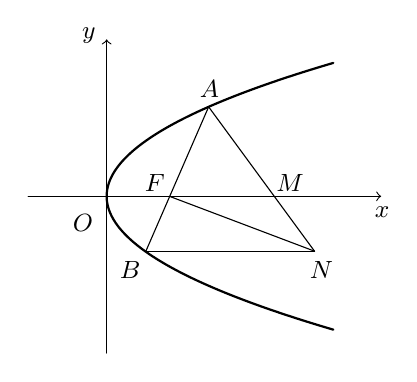
\begin{tikzpicture}[line cap=round,line join=round,font=\small,x=0.03515cm,y=0.03515cm]
% 坐标轴
\draw[->] (-28.33,0)--(99.18,0);
\draw[->] (0,-56.67)--(0,56.68);
% 抛物线（线宽 0.8，与源一致）
\draw[line width=0.8pt] plot[domain=-48.18:48.18,samples=121] ({\x*\x/28.35},{\x});
% ===== 直线段 =====
\draw (14.17,-19.83)--(36.84,32.31);   % A–B
\draw (14.17,-19.83)--(75.09,-19.83);  % B–N（水平）
\draw (36.84,32.31)--(75.09,-19.83);   % A–N
\draw (22.67,0)--(75.09,-19.83);       % F–N
% ===== 标注（照源字形框中心，显式坐标）=====
\node[anchor=center,inner sep=0] at (-6.39,58.10) {\(y\)};
\node[anchor=center,inner sep=0] at (37.11,38.74) {\(A\)};
\node[anchor=center,inner sep=0] at (17.39,4.73) {\(F\)};
\node[anchor=center,inner sep=0] at (66.30,4.73) {\(M\)};
\node[anchor=center,inner sep=0] at (99.47,-5.58) {\(x\)};
\node[anchor=center,inner sep=0] at (-8.58,-9.66) {\(O\)};
\node[anchor=center,inner sep=0] at (8.50,-26.45) {\(B\)};
\node[anchor=center,inner sep=0] at (77.64,-26.45) {\(N\)};
\end{tikzpicture}
\end{center}
\nopagebreak[4]
\end{question}
\begin{question}
\gkti{20}设函数 \(f(x)=x^{3}+\dfrac{1}{1+x}\)，\(x\in[0,1]\)。证明：

（1） \(f(x)\geqslant1-x+x^{2}\)；

（2） \(\dfrac{3}{4}<f(x)\leqslant\dfrac{3}{2}\)。

\end{question}